\chapter{EPRI-Style Load Separation in Abaqus} \label{chap:load-separation-epri}

%\section{EPRI-style Load Separation in Abaqus}

\todo[inline]{Conclusion: Abaqus models using fully plastic check blow up far too early to be useful except for materials that are close to perfectly-plastic? CMOD levels are way below what I got from WARP3D.}

\begin{figure}[tbp]
\centering
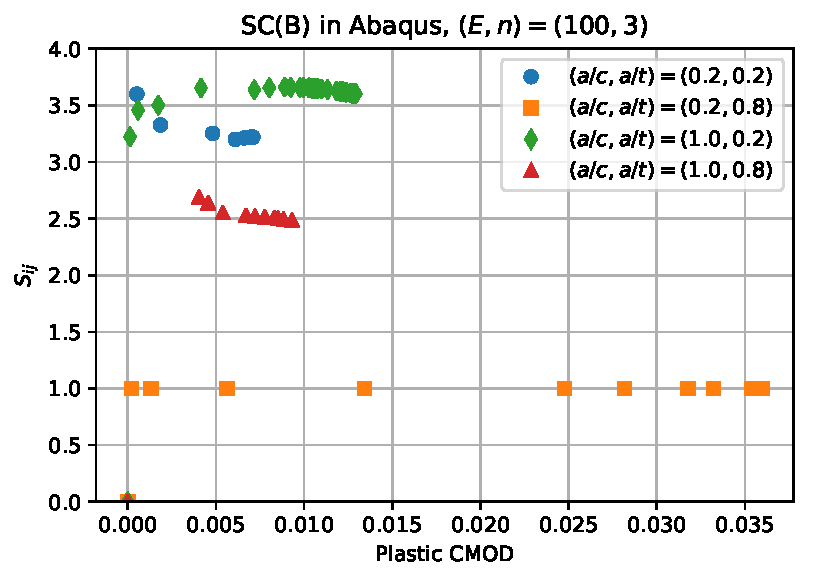
\includegraphics[width=0.8\columnwidth]{abaqus_bend_Sij_E0100_n03}
\caption{\Sij calculated from Abaqus (\(\frac{E}{\Sys}=100, n=3\))\label{fig:abaqus_Sij_E0100_n03}}
\end{figure}

\begin{figure}[tbp]
\centering
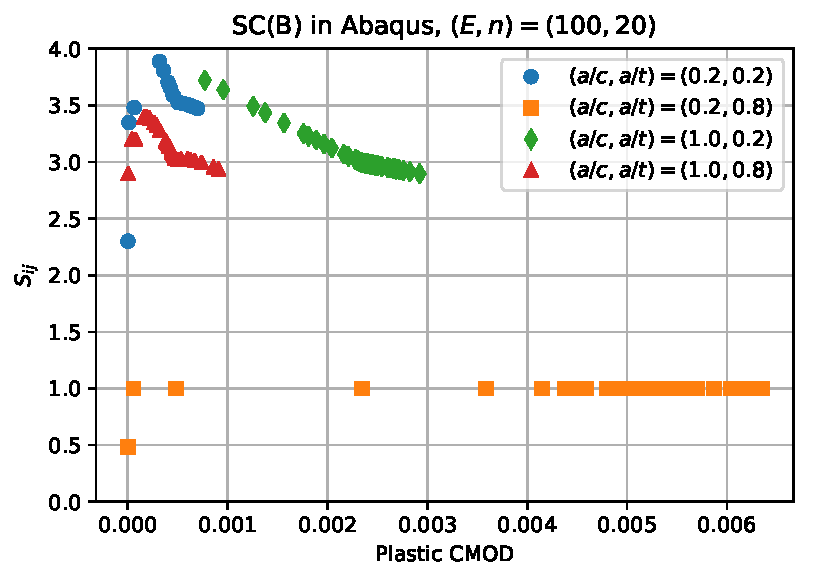
\includegraphics[width=0.8\columnwidth]{abaqus_bend_Sij_E0100_n20}
\caption{\Sij calculated from Abaqus (\(\frac{E}{\Sys}=100, n=20\))\label{fig:abaqus_Sij_E0100_n20}}
\end{figure}

\begin{figure}[tbp]
\centering
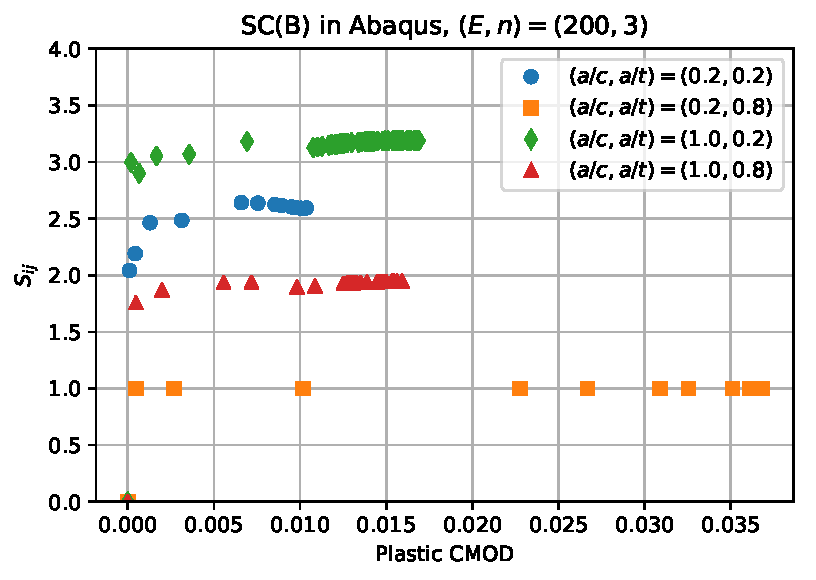
\includegraphics[width=0.8\columnwidth]{abaqus_bend_Sij_E0200_n03}
\caption{\Sij calculated from Abaqus (\(\frac{E}{\Sys}=200, n=3\))\label{fig:abaqus_Sij_E0200_n03}}
\end{figure}

\begin{figure}[tbp]
\centering
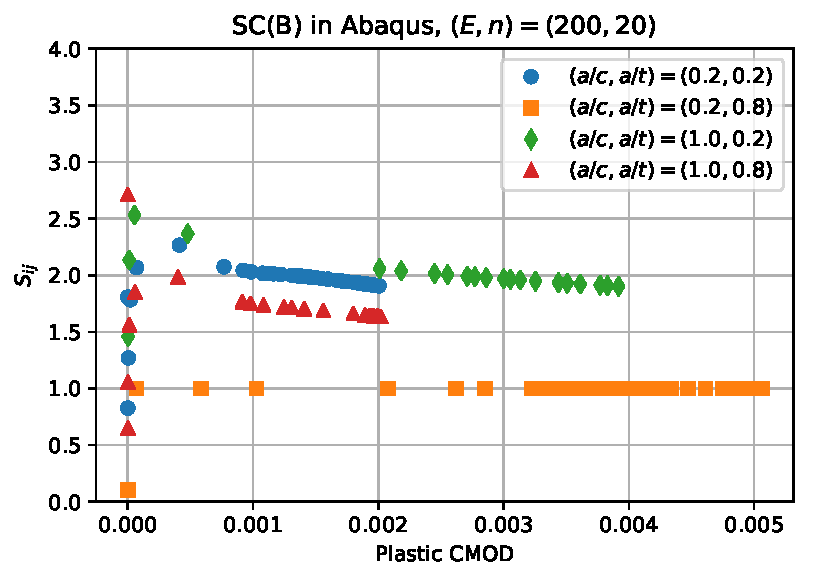
\includegraphics[width=0.8\columnwidth]{abaqus_bend_Sij_E0200_n20}
\caption{\Sij calculated from Abaqus (\(\frac{E}{\Sys}=200, n=20\))\label{fig:abaqus_Sij_E0200_n20}}
\end{figure}

\begin{figure}[tbp]
\centering
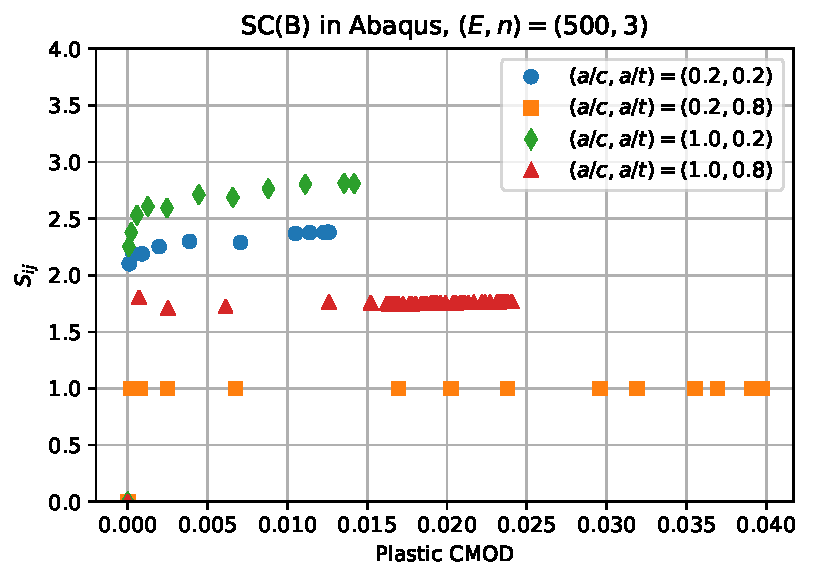
\includegraphics[width=0.8\columnwidth]{abaqus_bend_Sij_E0500_n03}
\caption{\Sij calculated from Abaqus (\(\frac{E}{\Sys}=500, n=3\))\label{fig:abaqus_Sij_E0500_n03}}
\end{figure}

\begin{figure}[tbp]
\centering
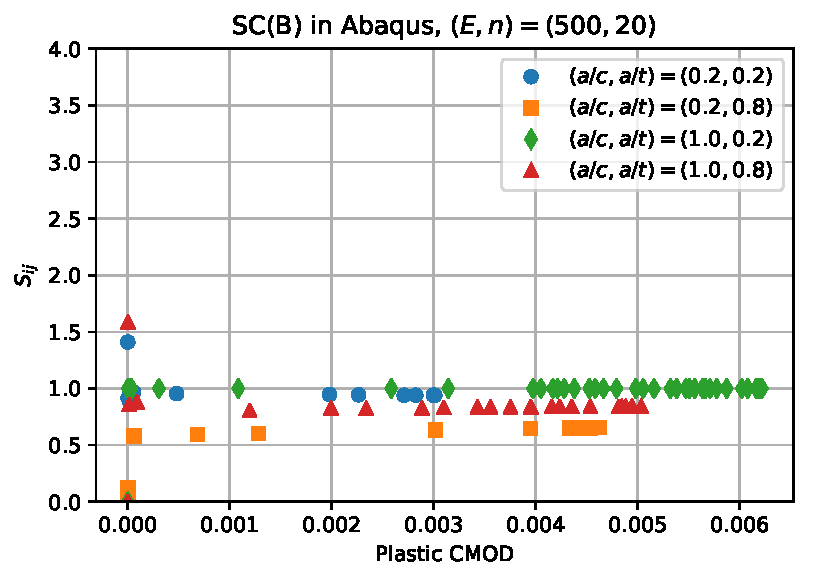
\includegraphics[width=0.8\columnwidth]{abaqus_bend_Sij_E0500_n20}
\caption{\Sij calculated from Abaqus (\(\frac{E}{\Sys}=500, n=20\))\label{fig:abaqus_Sij_E0500_n20}}
\end{figure}

\begin{figure}[tbp]
\centering
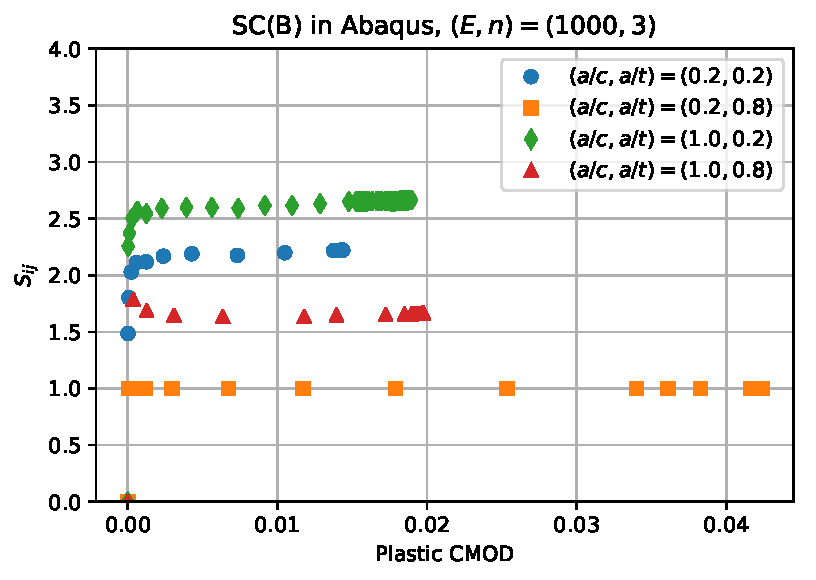
\includegraphics[width=0.8\columnwidth]{abaqus_bend_Sij_E1000_n03}
\caption{\Sij calculated from Abaqus (\(\frac{E}{\Sys}=1000, n=3\))\label{fig:abaqus_Sij_E1000_n03}}
\end{figure}

\begin{figure}[tbp]
\centering
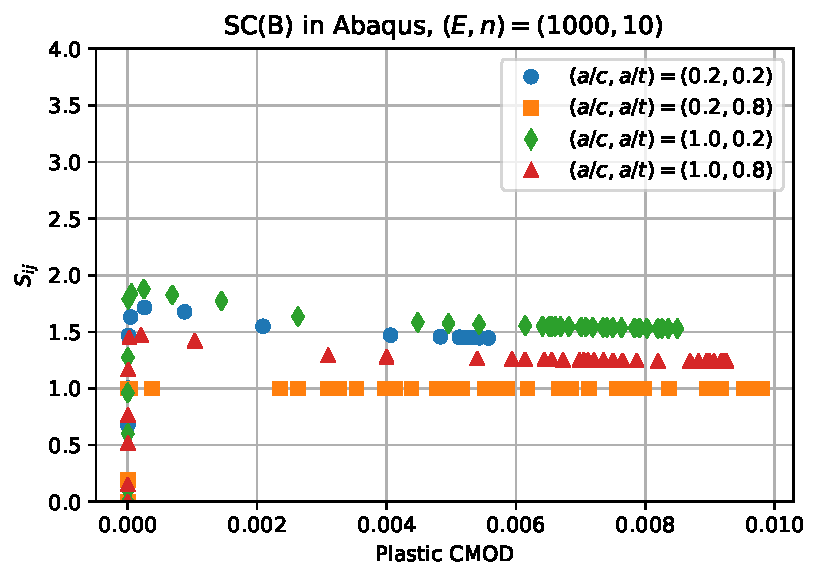
\includegraphics[width=0.8\columnwidth]{abaqus_bend_Sij_E1000_n10}
\caption{\Sij calculated from Abaqus (\(\frac{E}{\Sys}=1000, n=10\))\label{fig:abaqus_Sij_E1000_n10}}
\end{figure}

\begin{figure}[tbp]
\centering
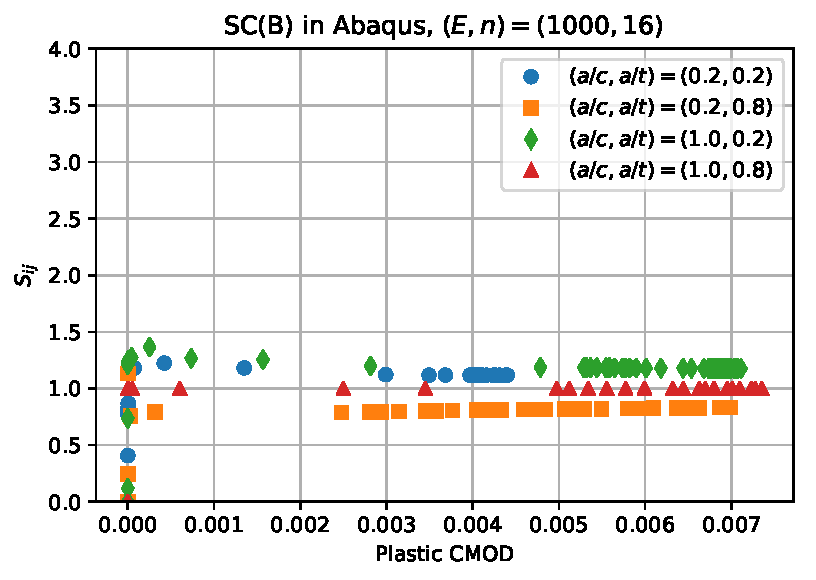
\includegraphics[width=0.8\columnwidth]{abaqus_bend_Sij_E1000_n16}
\caption{\Sij calculated from Abaqus (\(\frac{E}{\Sys}=1000, n=16\))\label{fig:abaqus_Sij_E1000_n16}}
\end{figure}

\begin{figure}[tbp]
\centering
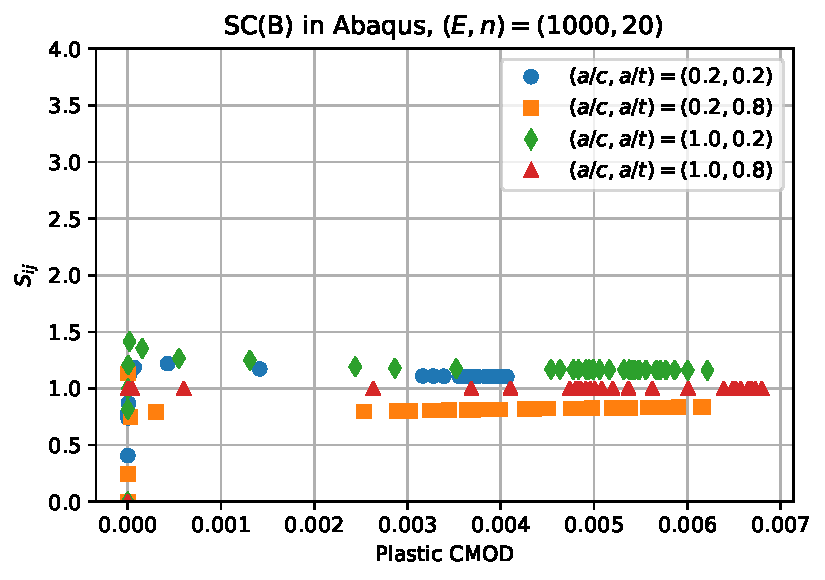
\includegraphics[width=0.8\columnwidth]{abaqus_bend_Sij_E1000_n20}
\caption{\Sij calculated from Abaqus (\(\frac{E}{\Sys}=1000, n=20\))\label{fig:abaqus_Sij_E1000_n20}}
\end{figure}

\begin{figure}[tbp]
\centering
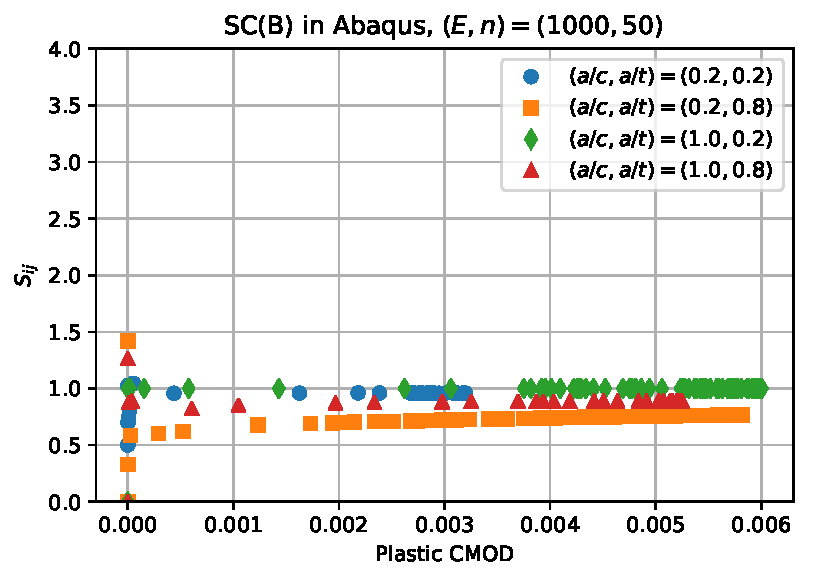
\includegraphics[width=0.8\columnwidth]{abaqus_bend_Sij_E1000_n50}
\caption{\Sij calculated from Abaqus (\(\frac{E}{\Sys}=1000, n=50\))\label{fig:abaqus_Sij_E1000_n50}}
\end{figure}
